\documentclass{standalone}
\usepackage{tikz}

\begin{document}
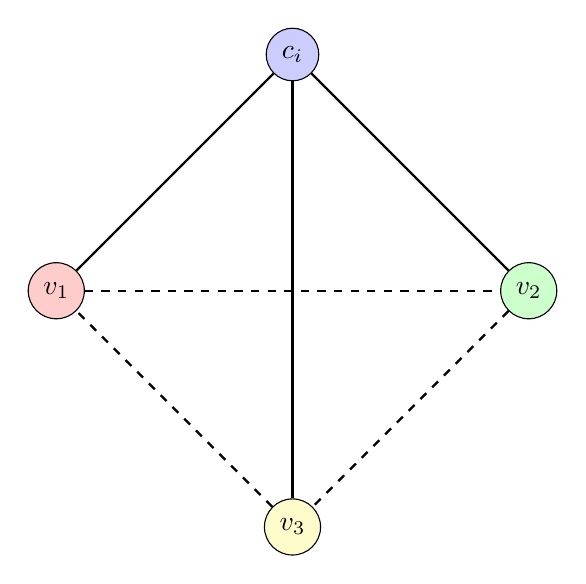
\begin{tikzpicture}[scale=1.5]

% Define the vertices
\node[circle, draw, fill=blue!20] (c1) at (0,0) {$c_i$};
\node[circle, draw, fill=red!20] (v1) at (-2,-2) {$v_1$};
\node[circle, draw, fill=green!20] (v2) at (2,-2) {$v_2$};
\node[circle, draw, fill=yellow!20] (v3) at (0,-4) {$v_3$};

% Draw the solid edges
\draw[thick] (c1) -- (v1);
\draw[thick] (c1) -- (v2);
\draw[thick] (c1) -- (v3);

% Draw the dashed edges
\draw[dashed, thick] (v1) -- (v2);
\draw[dashed, thick] (v2) -- (v3);
\draw[dashed, thick] (v3) -- (v1);

\end{tikzpicture}
\end{document}